
\section{Experiments}

\subsection{Training Details}
\label{sec:train_detail}

In this work, we focus specifically on mathematical tasks to evaluate our algorithm, which can be readily transferred to other tasks. We adopt the verl framework \cite{sheng2024hybridflow} for training. We use naive GRPO~\cite{deepseekmath} as our baseline algorithm and estimate advantages using group reward normalization.

For hyper-parameters, we utilize the AdamW \cite{loshchilov2018decoupled} optimizer with a constant learning rate of \(1 \times 10^{-6}\), incorporating a linear warm-up over 20 rollout steps.
For rollout, the prompt batch size is 512 and we sample 16 responses for each prompt. For training, the mini-batch size is set to 512, i.e., 16 gradient updates for each rollout step. For \textbf{Overlong Reward Shaping}, we set the expected maximum length as 16,384 tokens and allocate additional 4,096 tokens as the soft punish cache. Therefore, the maximum number of tokens for generation is set to 20,480 tokens. 
As for the \textbf{Clip-Higher} mechanism, we set the clipping parameter \(\varepsilon_{\text{low}}\) to 0.2 and \(\varepsilon_{\text{high}}\) to 0.28, which effectively balance the trade-off between exploration and exploitation.
For evaluation on AIME, we repeat the evaluation set for 32 times and report avg@32 for results stability. The inference hyperparameters of evaluation are set to temperature 1.0 and topp 0.7.
%The standard clip ratio $\epsilon$ is set to 0.2, while \(\epsilon_{\text{high}}\) for \textbf{Clip-Higher}, whereas \(\epsilon_{\text{low}}\) remains unchanged.

\begin{figure}[t]
    \centering
    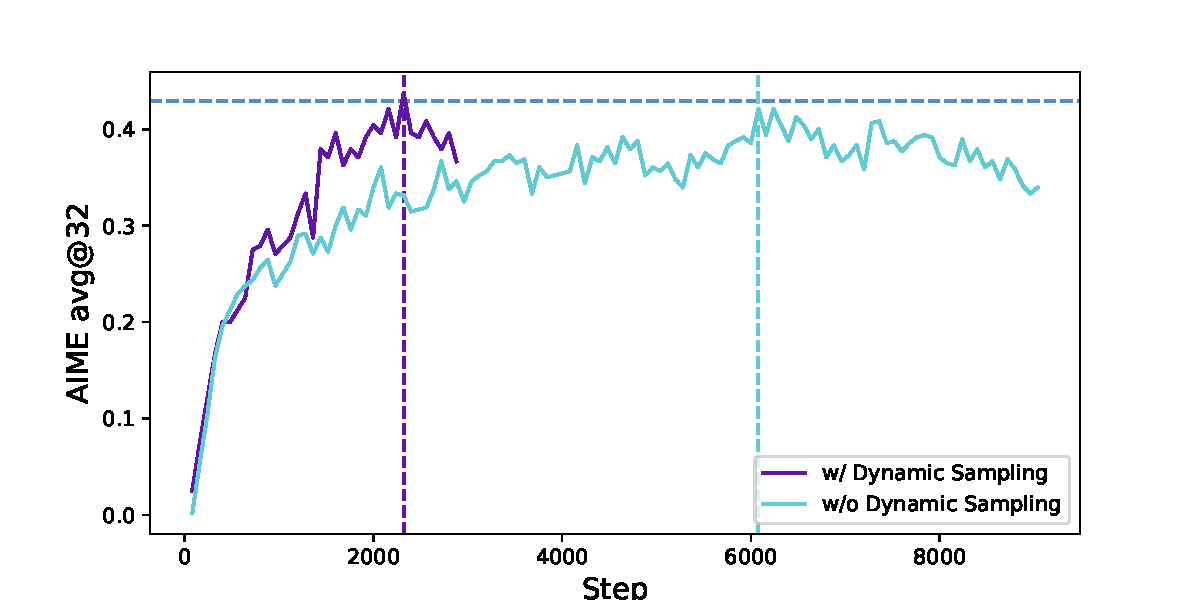
\includegraphics[width=0.7\linewidth]{figures/4.1.1.pdf}
    \caption{The training progress before and after applying dynamic sampling on a baseline setting.}
    \label{fig:afos_compare}
\end{figure}

\subsection{Main Results}

Experiments on AIME 2024 demonstrate that \method has successfully trained the Qwen-32B Base model into a powerful reasoning model, achieving performance superior to DeepSeek's experiments on Qwen2.5-32B using the R1 approach.
In Figure~\ref{fig:front}, we observe a substantial improvement of performance on AIME 2024, with accuracy increasing from near $0$\% to 50\%. Notably, this improvement is achieved with only 50\% of the training steps required by DeepSeek-R1-Zero-Qwen-32B.

We analyze the contributions of each training technique in our methodology, as detailed in \Cref{tab:results}.
The observed improvements demonstrate the effectiveness of these techniques in RL training, each contributing several accuracy points in AIME 2024.
Notably, given the vanilla GRPO setting, only 30\% accuracy can be reached by training from a Qwen2.5-32B base model.

For token-level loss, although it brings less performance improvement, we find it enhances training stability and makes the length increase more healthily.

When applying \textbf{Dynamic Sampling}, although more data needs to be sampled due to the filtering out of zero-gradient data, the overall training time is not significantly affected.
As shown in \Cref{fig:afos_compare}, although the number of sampling instances increases, the model's convergence time is even reduced, due to fewer training steps required.


\setcounter{table}{0}
\begin{table}[t]
    \centering
    \caption{Abalation results of \textbf{VAPO}}
    \begin{tabular}{l c}
        \toprule
        \textbf{Model} & $\textbf{AIME24}_\text{avg@32}$ \\
        \midrule
        Vanilla PPO & 5 \\
        \textbf{DeepSeek-R1-Zero-Qwen-32B}  & 47 \\
        \textbf{DAPO} & 50 \\
        \midrule
        VAPO w/o Value-Pretraining & 11 \\
        VAPO w/o Decoupled-GAE & 33 \\
        VAPO w/o Length-adaptive GAE & 45 \\
        VAPO w/o Clip-Higher & 46 \\
        VAPO w/o Token-level Loss & 53 \\
        VAPO w/o Positive Example LM Loss & 54 \\
        VAPO w/o Group-Sampling & 55 \\
        \textbf{VAPO} & \textbf{60} \\
        \bottomrule
    \end{tabular}
    \label{tab:results}
\end{table}


\subsection{Training Dynamics}

% It is essential to continuously monitor the metrics throughout the training process to ensure that improvements are quantified and any detriments are promptly addressed. 
% In Figure~\ref{fig:metrics}, we display the training curves of four important metrics: response length, reward score, generation entropy, and mean probability.
Reinforcement learning on large language models is not only a cutting-edge research direction but also an intrinsically complex systems engineering challenge, characterized by the interdependence of its various subsystems. Modifications to any single subsystem can propagate through the system, leading to unforeseen consequences due to the intricate interplay among these components. Even seemingly minor changes in initial conditions, such as variations in data and hyperparameters, can amplify through iterative reinforcement learning processes, yielding substantial deviations in outcomes. This complexity often confronts researchers with a dilemma: even after meticulous analysis and well-founded expectations that a modification will enhance specific aspects of the training process, the actual results frequently diverge from the anticipated trajectory. Therefore, monitoring of key intermediate results during experimentation is essential for swiftly identifying the sources of discrepancies and, ultimately, for refining the system. 

%% show some monitoring figures, and discusses our experience of debugging using through those monitoring

\begin{figure}[t]
    \centering
    \begin{subfigure}{0.45\textwidth}
        \centering
        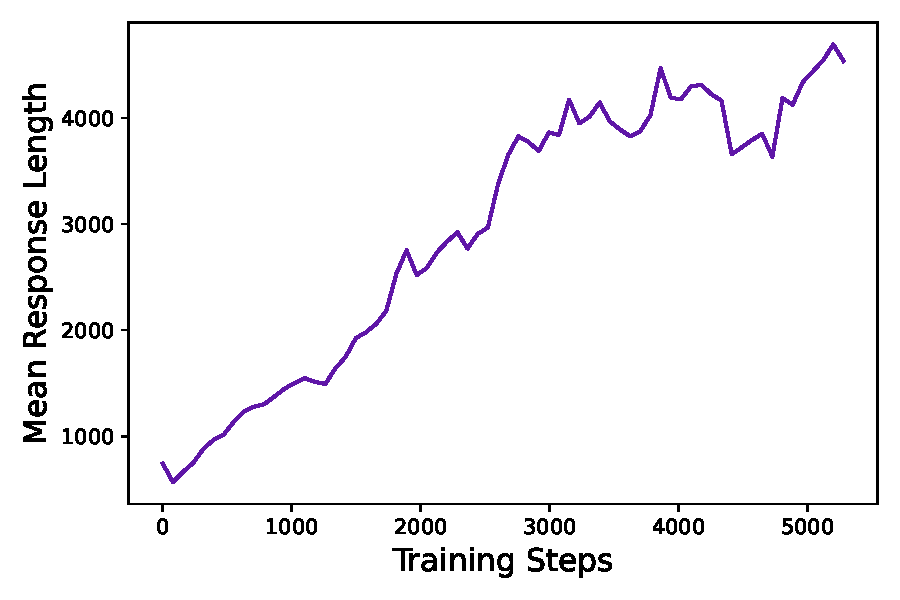
\includegraphics[width=\textwidth]{figures/length.pdf}
        % \captionsetup{labelformat=empty} % 只显示编号,不显示标题
        \caption{Mean response length.}
        \label{subfig:length}
    \end{subfigure}
    \hfill
    \begin{subfigure}{0.45\textwidth}
        \centering
        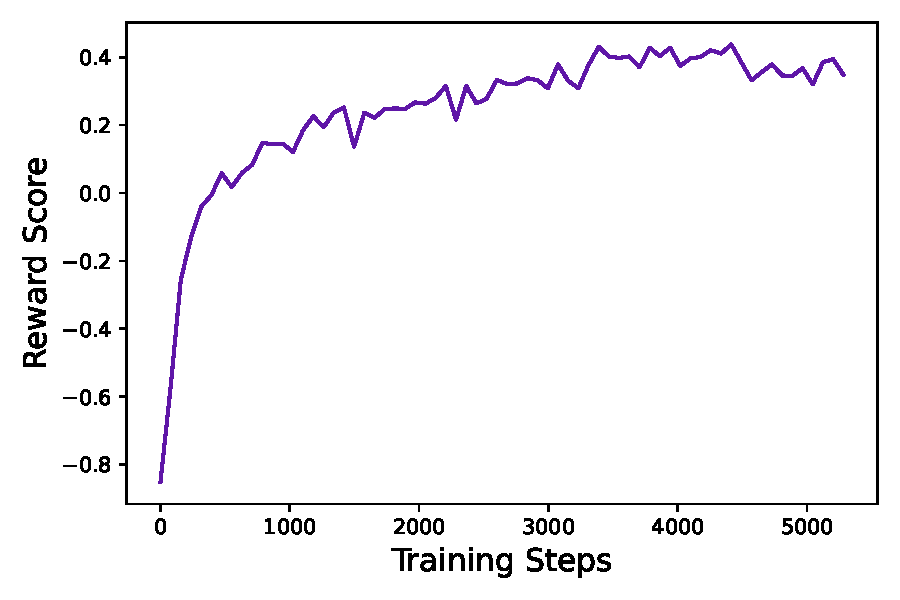
\includegraphics[width=\textwidth]{figures/reward.pdf}
        % \captionsetup{labelformat=empty} % 只显示编号,不显示标题
        \caption{Reward score.}
        \label{subfig:reward}
    \end{subfigure}
    \begin{subfigure}{0.45\textwidth}
        \centering
        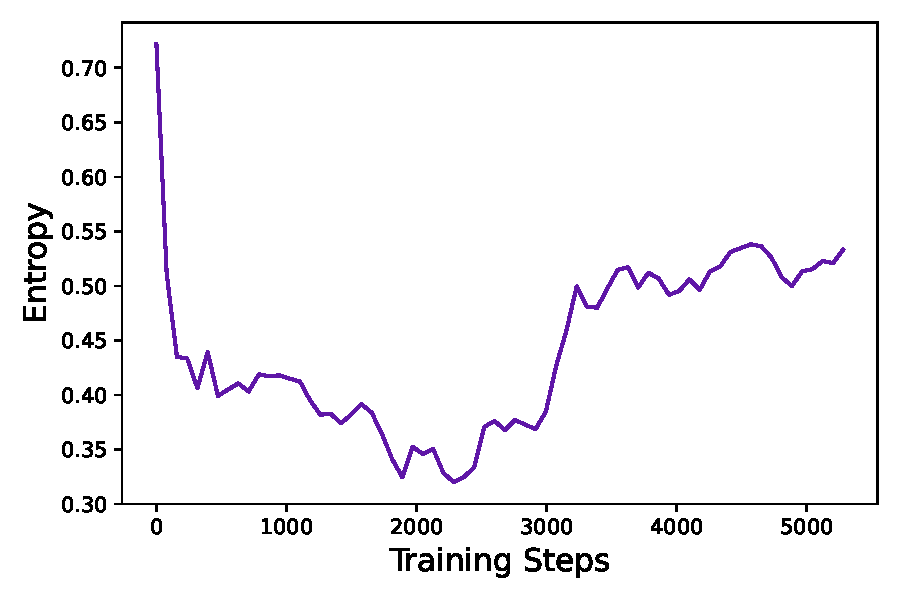
\includegraphics[width=\textwidth]{figures/entropy.pdf}
        % \captionsetup{labelformat=empty} % 只显示编号,不显示标题
        \caption{Generation entropy.}
        \label{subfig:entropy}
    \end{subfigure}
    \hfill
    \begin{subfigure}{0.45\textwidth}
        \centering
        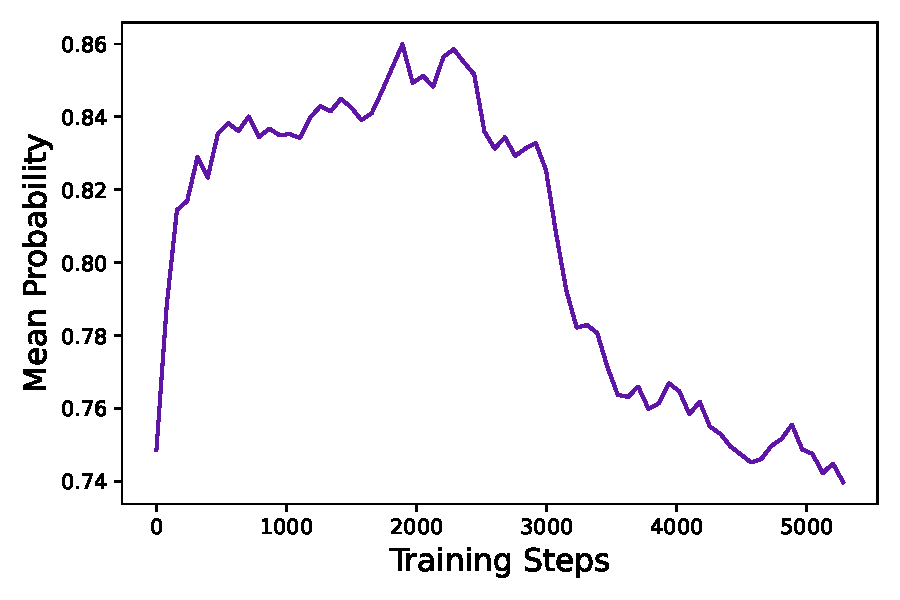
\includegraphics[width=\textwidth]{figures/prob.pdf}
        % \captionsetup{labelformat=empty} % 只显示编号,不显示标题
        \caption{Mean probability.}
        \label{subfig:prob}
    \end{subfigure}
    \caption{The metric curves of response length, reward score, generation entropy, and the mean probability of \method, which show the dynamics of RL training and serve as essential monitoring indicators to identify potential issues.}
    \label{fig:metrics}
\end{figure}

\begin{itemize}
\item 
% In reinforcement learning of reasoning models,
\textbf{The Length of Generated Responses} is a metric closely related to training stability and performance, as shown in \Cref{subfig:length}. The increase in length provides the model with a larger space for exploration, allowing more complex reasoning behaviors to be sampled and gradually reinforced through training. However, it is important to note that length does not always maintain a continuous upward trend during training. In some considerable periods, it can exhibit a trend of stagnation or even decline, which has also been demonstrated in \cite{guo2025deepseek}. We typically use length in conjunction with validation accuracy as indicators to assess whether an experiment is deteriorating.

\item \textbf{The Dynamics of Reward} during training has always been one of the crucial monitoring indicators in reinforcement learning, as shown in \Cref{subfig:reward}. In the majority of our experiments, the trend of reward increase is relatively stable and does not fluctuate or decline significantly due to adjustments in experimental settings. This indicates that, given a reliable reward signal, language models can robustly fit the distribution of training set. However, we find that the final reward on the training set often exhibits little correlation with the accuracy on the validation set, which indicates overfitting to the training set.

\item \textbf{The Entropy of the Actor Model and Generation Probability} are related to the model's exploration capability and are key metrics that we closely monitor in our experiments. Intuitively, the model's entropy needs to be maintained within an appropriate range. An excessively low entropy indicates that the probability distribution is overly sharp, leading to a loss of exploration capability. Conversely, an excessively high entropy is often associated with issues of over-exploration such as gibberish and repetitive generation. For the generation probability, the situation is exactly the opposite. As demonstrated in \Cref{sec:cliphigher}, by applying the Clip-Higher strategy, we effectively addressed the issue of entropy collapse. In subsequent experiments, we find that maintaining a slow upward trend in entropy is conducive to the improvement of model performance, shown in \Cref{subfig:entropy} and \Cref{subfig:prob}.
\end{itemize}

\subsection{Case Study}
% an example, show perforance gains (responses) before and after RL training.
% an example, show that before and after applying some metric (clip-high), how the 

% \begin{table}[h]
%     \centering
%     \begin{minipage}[t]{0.50\textwidth}
%         \centering
%         \begin{tabular}{@{}p{\textwidth}@{}}
%             \toprule
%             Row 1 content here... \\
%             \midrule
%             Row 2 content here... \\
%             \bottomrule
%         \end{tabular}
%         \caption{Table 1}
%         \label{tab:table1}
%     \end{minipage}
%     \hfill % 添加一些间距
%     \begin{minipage}[t]{0.50\textwidth}
%         \centering
%         \begin{tabular}{@{}p{\textwidth}@{}}
%             \toprule
%             Row 1 content here... \\
%             \midrule
%             Row 2 content here... \\
%             \bottomrule
%         \end{tabular}
%         \caption{Table 2}
%         \label{tab:table2}
%     \end{minipage}
% \end{table}

\begin{table}[h]
    \centering
    \begin{tabular}{@{}p{0.9\textwidth}@{}} 
        \toprule 
        \textbf{Question}: \\
        Given that the base $ABC$ of the tetrahedron $S-ABC$ is an equilateral triangle, the projection $H$ of point $A$ on the face $SBC$ is the orthocenter of $\triangle SBC$, the dihedral angle $H-AB-C$ is $30^\circ$, and $SA = 2$, find the volume of the tetrahedron. The answer is in the form $\frac{k}{m}$, so give the value of $k+m$.\\
        \midrule 
        \textbf{Response}: \\
        Let us consider the given problem: We need to determine ... \\
        ... \\
        Next, let $S$ have coordinates $(x_0, y_0, z_0)$. Since $SA=2$, the distance formula gives us $\sqrt{(x_0)^2 + (y_0)^2 + (z_0)^2}= 2$, so we can write $x_0^2 + y_0^2 + z_0^2= 4$. Now, remember that $H$ is the orthogonal projection of\\
        ... \\
        \textcolor{red}{However, wait a moment, let's rethink about the dihedral angle involving planes in a more thoughtful geometric way.} Consider the plane $\alpha_1=ABC$, which lies entirely on the xy coordinate plane (as $z = 0$). Let the plane $\alpha_2=SBC$. The point $A$ projected perpendicularly to plane $\alpha_2$ lands on $H$. The line $l=AB$ ...\\
        ... \\
        \bottomrule
    \end{tabular}
    \caption{Emergence of Reflective Behavior in Reinforcement Learning}
    \label{tab:case_study1}
\end{table}

% During the RL training process, linguistic patterns that aid in solving complex problems are progressively enhanced.
% In addition, we found that certain modes of reasoning, which were virtually absent at the beginning of training, gradually emerged as training progressed.
During the RL training process, we observe an interesting phenomenon: the reasoning patterns of the actor model evolve dynamically over time. Specifically, the algorithm not only reinforces existing reasoning patterns that facilitate correct problem-solving but also gradually gives rise to entirely new modes of reasoning that were initially absent.
This finding reveals the adaptability and exploration capability of RL algorithms and offers new insights into the learning mechanisms of the model.

For example, in the early stages of model training, there was virtually no occurrence of checking and reflecting on previous reasoning steps.
However, as training progresses, the model exhibits distinct behaviors of reflection and backtracking, as shown in \Cref{tab:case_study1}. This observation sheds light on further exploration into interpreting the emergence of reasoning abilities during RL, which we leave for future research.

% This further illustrates the immense potential of reinforcement learning compared to supervised learning: by providing explicit incentives rather than instructing the model on what to do, the actor model is able to explore unexpected problem-solving paths by maintaining a delicate balance between exploration and exploitation.

% \begin{table}[h]
%     \centering
%     \begin{tabular}{@{}p{0.9\textwidth}@{}} 
%         \toprule 
%         Question:  \\
%         \midrule 
%         Response... \\
%         \bottomrule 
%     \end{tabular}
%     \caption{Emergence of reflective behavior in reinforcement learning.}
%     \label{tab:case_study1}
% \end{table}

% \begin{table}[h]
\centering
\caption{Leave-One-Out Ablations}
\label{tab:leave-one-out_ablation}
\begin{tabular}{l c}
\toprule
\textbf{Setting} & $\textbf{AIME24}_\text{avg@32}$
\\
\midrule
\method & --\\
\midrule
\ \  w/o Clip-Higher Strategy & -- \\
\ \  w/o Token-Level Policy Gradient Loss & --\\
\ \  w/o Reward Shaping & -- \\
\ \  w/o Gradient-Keeping Strategy & -- \\
\bottomrule
\end{tabular}%
\end{table}


% To validate the efficacy of our RL training recipe, we conduct ablation experiments where we leave out all but one of the aforementioned adjustments. The results are shown in Table~\ref{tab:leave-one-out_ablation}.
